\section{Introduction}
\label{Introduction}
The alignment of Large Language Models (LLMs) with human feedback, as explored in works like GPT-4 and LLaMA-2 \cite{GPT4,llama2,GPT4_2}, has marked a significant advancement in generating responses that are more helpful, factual, and ethical \cite{instructGPT}. Among the various alignment strategies, Reinforcement Learning from Human Feedback (RLHF) \cite{instructGPT} is a notable method that refines LLMs using the Proximal Policy Optimization (PPO) algorithm \cite{PPO}. This approach employs a KL divergence penalty to ensure minimal deviation of the model from its original configuration, ensuring the retention of its initial characteristics while improving alignment.

Despite the effectiveness, RLHF's instability and computational requirements often limit its practical applications, prompting the exploration of alternatives like Direct Preference Optimization (DPO) \cite{DPO}. DPO circumvents the reinforcement learning loop by exploiting the inherent connection between reward functions and optimal policies, thereby simplifying the policy model training. It encourages the model to favor the response that aligns with human preferences ($\yb_{w}$) over the dispreferred ($\yb_{l}$), \wjc{implying DPO's sensitivity to the quality of pairwise data}. 
The balance between maintaining the original reference model ($\pi_{\text{ref}}$) and incorporating new preferences ($\pi_{\btheta}$) is controlled by a $\beta$ hyperparameter, whose lower values advocate for aggressive updates and higher values support more conservative adjustments:
\begin{align*}
    \ell_{\text{DPO}}(\btheta)=\EE_{\xb,\yb_{w},\yb_{l}} [-\log \sigma \big(
    \beta \big[
    \log \big(\frac{\pi_{\btheta}(\yb_{w}|\xb)}{\pi_{\text{ref}}(\yb_{w}|\xb)}\big)
    -
    \log \big(\frac{\pi_{\btheta}(\yb_{l}|\xb)}{\pi_{\text{ref}}(\yb_{l}|\xb)}\big)
    \big]
    \big)].
\end{align*}
However, the current DPO literature has largely overlooked the joint influence of $\beta$ selection and pairwise data $(\yb_{w}, \yb_{l})$'s quality on the alignment performance.
\wjc{To bridge this gap, we conduct a preliminary experiment to investigate how different $\beta$ selections influence the model performance under two distinct data pair gap conditions, as shown in Figure \ref{fig_1_2}.}
In \emph{low gap} scenarios (\cf Figure \ref{fig_1_1}),
where the difference between preferred and dispreferred samples is minor, an increase in $\beta$ (\eg from 0.1 to 0.5) corresponds with a decline in win rate (\eg from 42\% to 33\%).
Conversely, in \emph{high gap} situations (\cf Figure \ref{fig_1_1})
where a significant difference exists, an increase in $\beta$ tends to improve DPO performance.
\wjc{Such contrasting outcomes highlight the necessity to tailor the $\beta$ value contingent upon the data quality, especially in the presence of outliers \cite{outlier_dataset}.}
\begin{figure}
    \centering
    \begin{subfigure}{.65\textwidth}
      \centering
      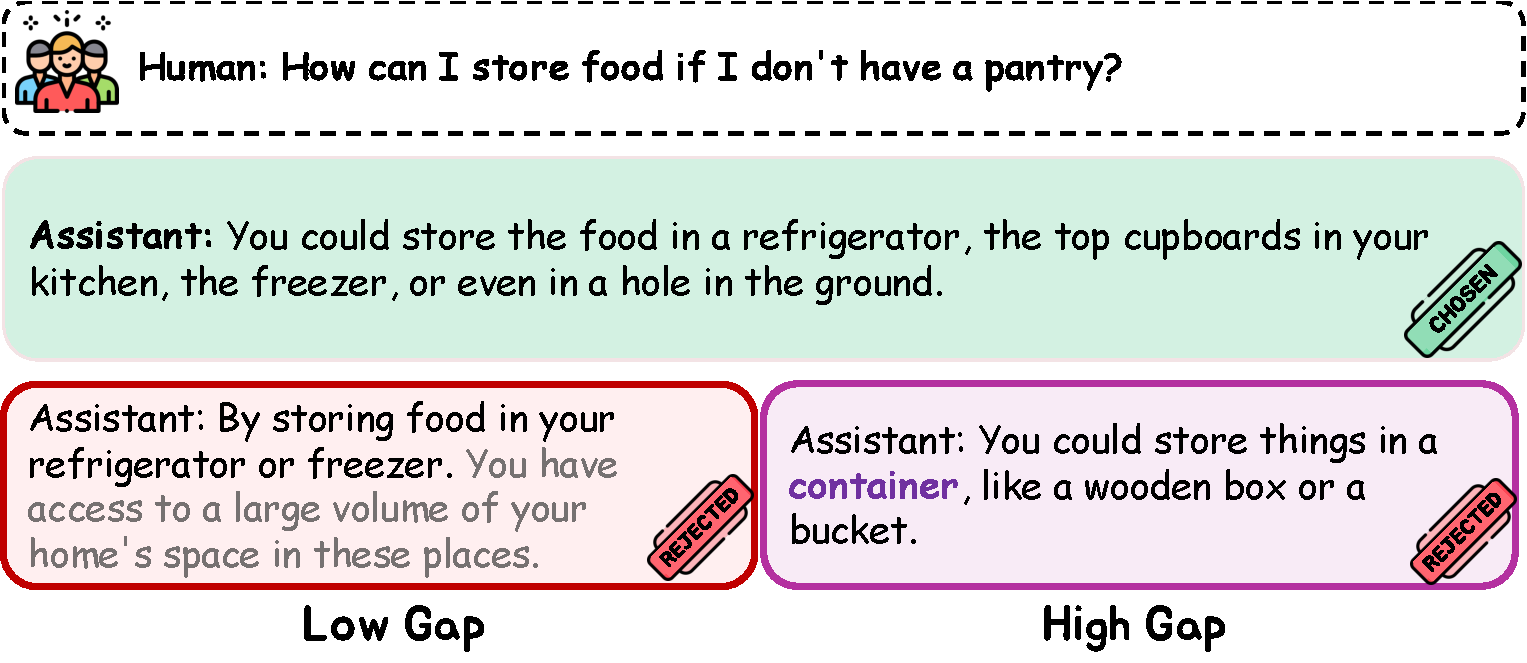
\includegraphics[width=\linewidth]{figs/first_fig_a.pdf}
      \caption{} % 你可以在这里添加子图标题
      \label{fig_1_1}
    \end{subfigure}%
    \hfill % 这会在子图之间添加一些空间
    \begin{subfigure}{.3\textwidth}
      \centering
      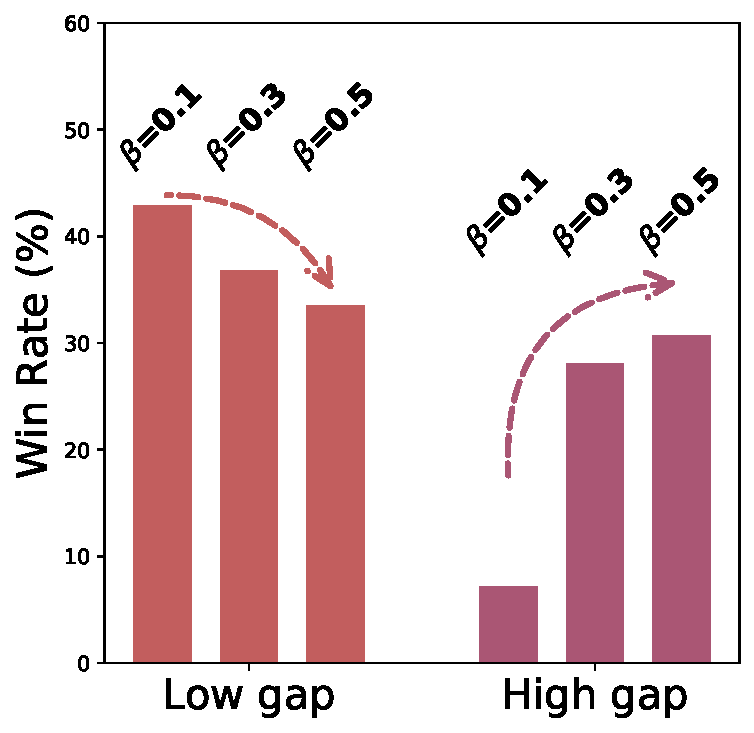
\includegraphics[width=\linewidth]{figs/NeurIPS_first_fig.pdf}
      \caption{} % 同样,为第二个子图添加标题
      \label{fig_1_2}
    \end{subfigure}
    \caption{
    \textbf{(\ref{fig_1_1}) Pairwise Data: Low vs. High Gap}: ``Low gap'' denotes cases where the chosen and rejected examples are closely similar, typically indicating high-quality, informative pairs. ``High gap'' signifies pairs with larger differences, implying lower-quality data.
    \textbf{(\ref{fig_1_2}) Influence of Data Quality on $\beta$ Selection:} Pythia-1.4B's performance on the HH dataset reveals a distinct trend: for ``Low gap'', a higher $\beta$ reduces win rate, whereas for ``High gap'', an increased $\beta$ improves it.}
    \label{fig:combined}
\end{figure}

Building upon these insights and recognizing the mixture nature of diverse quality in practically collected data \cite{mixture_data},
we propose a dynamic $\beta$ selection strategy for DPO. This strategy adaptively adjusts $\beta$ in response to the quality of pairwise data and robustifies DPO against data variability. 
Intuitively, one straightforward solution is personalizing $\beta$ for each pair, rather than fixing it across the population of all pairs. While conceptually appealing, (1) instance-level $\beta$ personalization can lead to optimization instabilities, particularly when dealing with a vast array of human preference instances \wjc{(\cf Section \ref{sec_batch_level})}. This issue underscores the challenge of balancing $\beta$ updates with stable and scalable DPO. In this light, we propose to explore a \textit{batch-level} adaptation of $\beta$, aiming to balance update aggressiveness and training stability. Moreover, (2) the frequent occurrence of outliers necessitates a strategy for accurately adjusting the batch-level $\beta$. 
The dataset notably features outliers, a challenge underscored by the significant reward discrepancy variations within the training samples of the dataset (\cf Section \ref{motivation_sec}). 
Such conditions impede the model's ability to accurately estimate the batch-level $\beta$, thereby undermining the effectiveness of batch-level $\beta$ calibration.
To this end, we propose a simple yet effective dual-component approach:


\begin{itemize}[leftmargin=*]
  \item \textbf{Dynamic $\beta$ Calibration at Batch-Level} (for Challenge 1): To mitigate optimization instabilities, we dynamically calibrate $\beta$ within each batch. Specifically, this batch-level adjustment is based on data quality, with $\beta$ being adaptively decreased for high-quality, closely-matched pairwise data (\ie \emph{low gap} data) to facilitate assertive updates. While for easily-discriminated pairs (\ie \emph{high-gap} data), $\beta$ is increased to promote cautious updates, preventing overfitting to noise.
  This targeted batch-level calibration enables stable and responsive optimization.
  \item \textbf{$\beta$-Guided Data Filtering} (for Challenge 2): We implement a $\beta$-guided data filtering approach to tackle the frequent occurrence of outliers. By establishing a benchmark $\beta$ value for filtering incoming data at the batch level, we maintain the fidelity of $\beta$ estimation by prioritizing the most reliable and representative samples. As a result, it diminishes the impact of outliers that might otherwise derail the optimization process, thus enhancing the precision and robustness of the batch-level $\beta$ calibration.
\end{itemize}

Our contributions are threefold: (1) We investigate a pioneering study on the joint influence of $\beta$ selection and pairwise data quality on the DPO performance. (2) We introduce a simple yet effective $\beta$-dynamic strategy for DPO, adaptively balancing the update aggressiveness and training stability. (3) Through empirical evaluations, our approach demonstrates marked improvements in performance across diverse conditions and model sizes
(\eg achieving improvements exceeding 10\% on models of various sizes, including Pythia-410M, 1.4B, and 2.8B).

% To navigate these challenges, our research introduces a dual-optimization strategy: first, dynamically adjusting $\beta$ at the batch level according to the data quality and second, employing a filtration mechanism that leverages a benchmarked $\beta$ to reduce outlier interference. We pioneer in unraveling the relation between $\beta$ parameters and pairwise data quality, suggesting an innovative and adaptable solution. Our empirical validation across diverse settings and model sizes confirms that this dynamic $\beta$ strategy enhances performance significantly.

% Our contributions are threefold: (1) We present a pioneering study on how the quality of pairwise data influences the choice of $\beta$. (2) We introduce a novel dynamic $\beta$ mechanism, responsive to data quality. (3) Through empirical evaluations, our approach demonstrates marked improvements in performance across diverse conditions and model sizes.

% This paper proposes a dynamic approach to the $\beta$ parameter in DPO, aiming to adapt to a diverse range of preference data. We identify two principal challenges in implementing dynamic $\beta$: the risk of unstable optimization when assigning unique $\beta$ values to individual data instances, and the influence of outliers when determining batch-level $\beta$ settings. To innovate within these constraints, we devise a dual optimization strategy:


% \textbf{Dynamic $\beta$ Calibration with Batch-Level Adaptation:} This mechanism dynamically calibrates the $\beta$ value in response to the quality of pairwise preference data. By evaluating the proximity between preferred responses and their references, $\beta$ is decreased to encourage more assertive updates when the data indicates a close match and high quality (\emph{low gap}). Conversely, in cases where the data exhibits a \emph{High gap}, $\beta$ is increased to endorse more conservative updates, safeguarding against potential overfitting to noisy or less informative data.

% \textbf{$\beta$-Guided Data Filtering:} To enhance the accuracy of $\beta$ calibration and mitigate the effects of outliers, we implement a selective data filtering process. This method utilizes a benchmark $\beta$ value to screen the incoming data at the batch level, ensuring that the estimation of $\beta$ is based on the most reliable and representative samples. Consequently, this assists in reducing the influence of outliers that could otherwise skew the optimization trajectory.

% \textbf{Beta Quality Adjustment:} The $\beta$ value adjusts based on the proximity between preferred responses and references, promoting more vigorous updates in scenarios with close-mapped high-quality data (Low Gap) and maintaining cautious updates in the presence of broader gaps (High Gap).

% \textbf{Data Filtering:} A filtering process is employed to refine the influence of outliers on $\beta$ estimation at the batch level.



% Our empirical inquiry reveals the nuanced influence of (\beta)'s magnitude on DPO's generative performance. As depicted in Figure \ref{fig_1_2} (red bars), altering (\beta) from 0.1 to 0.5 correlates with a reduction in win rate, declining notably from 42\% to 33\%—a testament to the delicate interplay between hyperparameter tuning and model output. This sensitivity is further modulated by the quality of training pairs, a factor we corroborate quantitatively. Data pairs exhibiting a \emph{low gap} generally convey a high informational content, fostering a setting where a reduced (\beta) bolsters effective policy learning. In stark contrast, when confronted with a \emph{high gap}, indicative of sparse information, a conservative (\beta) is prudent to avoid overfitting trivial discrepancies. The optimal calibration of (\beta) thus navigates a spectrum conditioned by data quality differentiation, as evidenced by our comparison between different gap levels (purple bars in Figure \ref{fig_1_2}). The shifting landscape of (\beta) efficacy, especially in settings rife with outliers, underscores the inadequacy of static (\beta) application within the DPO framework.

% Our investigations reveal that the performance of DPO is intricately linked with the selection of the $\beta$ parameter and the quality of the training pairs. Notably, typical practice often defaults $\beta$ to a static value, for instance, 0.1. However, as our empirical findings depict in Figure \ref{fig_1_2} (red bars), such a one-size-fits-all approach may not be ideal. The generative capacity of DPO showcased marked variations with adjustments in $\beta$; an increase from 0.1 to 0.5 led to a pronounced drop in the win rate, plummeting from 42\% to 33\%. This sensitivity is further complicated by the inherent quality of the data, where we witness the optimal selection of (\beta) shifting in response to the nature of the training pairs evaluated. The low gap versus high gap comparison elucidates this dynamic, with optimum $\beta$ values diverging under different data quality scenarios, as illustrated by the purple bars in Figure \ref{fig_1_2}.

% This empirically informed perspective underscores a critical observation — statically fixed (\beta) values are suboptimal for DPO in real-world scenarios marred by data variability and outliers. For example, training pairs closely aligned (\emph{low gap}) are rich in informative content, demanding a lower (\beta) to facilitate effective policy updates. Conversely, pairs with significant dissimilarities (\emph{high gap}) prompt a higher (\beta), mitigating the risk of overfitting on potentially less informative examples. Such nuanced understanding, enabled by our data-driven analysis, sets the stage for a dynamically adapted (\beta), tailored to the batch-specific characteristics and tackling the variability presented by outliers head on.

% Often, the $\beta$ value is typically set to a fixed value, such as $0.1$. But, the generative performance of DPO exhibits a marked sensitivity to the parameter $\beta$, as illustrated in Figure \ref{fig_1_2} (red bars). Notably, when $\beta$ is increased from 0.1 to 0.5, we observe a decline in the win rate from 42\% to 33\%. And the optimal selection of $\beta$ is subject to shift due to variations in data quality (purple bars in \ref{fig_1_2}). For alignment, informative and high quality pairwise data are intuitively those pairs that are mapped nearby (low gap between $\yb_{w}$ and $\yb_{l}$) but should be far apart. By comparing pairs of ($\yb_{w},\yb_{l}$) at different levels of gap (low gap vs. high gap), it is observed that the optimal value of $\beta$ alters correspondingly. Consequently, given the presence of variability in data quality (i.e., outliers) in real-world scenarios, \emph{a fixed $\beta$ is no longer the optimal choice for the DPO.}

% Empirical evidence suggests that the optimal $\beta$ is sensitive not just to its selection but also to the nature of the training pairs. When too close (\emph{low gap}), the pairs harbor rich information, necessitating a lower $\beta$ for effective policy updates. Conversely, when pairs are evidently disparate (\emph{high gap}), a conservative $\beta$ avoids overfitting on less informative examples. The influence of data variability, especially outliers, becomes significant in real-world distributions, invalidating a static $\beta$ choice.

% Motivated by this, we propose a dynamic selection of $\beta$, which is informed by the quality of pairwise data and addresses data variability robustly. The implementation of this strategy introduces two key challenges: (1) instance-wise $\beta$ attribution can lead to optimization instabilities, and existing population-level approaches do not suffice. Therefore, we propose a batch-level adaptation of $\beta$, balancing update aggressiveness and training stability. (2) The prevalence of outliers necessitates a method to identify and adjust the batch-level $\beta$ appropriately.

% To navigate these challenges, our research introduces a dual-optimization strategy: first, dynamically adjusting $\beta$ at the batch level according to the data quality and second, employing a filtration mechanism that leverages a benchmarked $\beta$ to reduce outlier interference. We pioneer in unraveling the relation between $\beta$ parameters and pairwise data quality, suggesting an innovative and adaptable solution. Our empirical validation across diverse settings and model sizes confirms that this dynamic $\beta$ strategy enhances performance significantly.

% Aligning Large Language Models (LLMs) \cite{GPT4,llama2,GPT4_2} with human feedback has become a critical step to ensure that their outputs are helpful, factual, and ethical \cite{instructGPT}. Despite the effectiveness of Reinforcement Learning from Human Feedback (RLHF) \cite{instructGPT} using the Proximal Policy Optimization (PPO) algorithm \cite{PPO}, it incurs non-negligible costs in terms of stability and computational demand compared to supervised methods. This approach utilizes a reverse KL divergence penalty to guarantee the modeled behavior does not significantly stray from its trained foundation.

% Direct Preference Optimization (DPO) \cite{DPO} has emerged as a promising alternative, streamlining alignment by bypassing complex RL procedures. DPO directly maps preferences, leveraging pairwise comparisons between human-favored responses $\yb_{w}$ and reference responses $\yb_{l}$. The hyperparameter $\beta$ modulates the inclination towards the preferred responses by adjusting the policy model's updates. However, surprisingly, considerations regarding the choice of $\beta$ and the quality of pairwise preference data have been overlooked in existing DPO applications.

% This paper proposes a dynamic approach to the $\beta$ parameter in DPO, aiming to adapt to a diverse range of preference data. We identify two principal challenges in implementing dynamic $\beta$: the risk of unstable optimization when assigning unique $\beta$ values to individual data instances, and the influence of outliers when determining batch-level $\beta$ settings. To innovate within these constraints, we devise a dual optimization strategy:

% \textbf{Beta Quality Adjustment:} The $\beta$ value adjusts based on the proximity between preferred responses and references, promoting more vigorous updates in scenarios with close-mapped high-quality data (Low Gap) and maintaining cautious updates in the presence of broader gaps (High Gap).

% \textbf{Data Filtering:} A filtering process is employed to refine the influence of outliers on $\beta$ estimation at the batch level.

% Our contributions are threefold: (1) We present a pioneering study on how the quality of pairwise data influences the choice of $\beta$. (2) We introduce a novel dynamic $\beta$ mechanism, responsive to data quality. (3) Through empirical evaluations, our approach demonstrates marked improvements in performance across diverse conditions and model sizes.



% DPO relies on two key ingredients: the selection of $\beta$ and the quality of pairwise data. The training objective guides the policy model to prefer the human-preferred action over the reference action by a margin. The $\beta$ value is a hyperparameter that controls the deviation from the base reference policy $\piref$. A smaller $\beta$ value leads to a more aggressive update, while a larger $\beta$ value leads to a more conservative update. 

% The quality of the pairwise data is crucial for the model to learn effectively. In the context of DPO, the quality of the pairwise data is assessed by the reward differences between the sample pairs. When the pairwise data is of high quality, a small and fixed $\beta$ is sufficient to achieve good performance. However, when the pairwise data is of poor quality or not all high quality, the small and fixed $\beta$ will lead to overfitting.


% Therefore, the methodology advanced here is keenly attuned to outlier detection and management, ensuring the integrity of the batch-optimized beta determination.

% To 
% In this work, we employ a \textit{danamic} $\beta$ during training and 
% And the pairwise data are assumed to be of high quality. 

% However, the optimal $\beta$ value is contingent upon the quality of the pairwise data. When the pairwise data is of high quality, a small and fixed $\beta$ is sufficient to achieve good performance. However, when the pairwise data is of poor quality or not all high quality, the small and fixed $\beta$ will lead to overfitting. In this paper, we propose a method to estimate a better $\beta$ that upholds Principle 1, and simultaneously combines this idea with data filtering to address Principle 2.
% leverages the mapping between the reward
% function and the optimal policy to bypass the need for reinforcement learning and explicit reward
% model learning.
% has emerged as an alternative

% Despite the DPO has exhibited exceptional performance across a variety of tasks, we remain intrigued by the potential to maximize the capabilities of DPO. To this end, our inquiry is particularly focused on two aspects: the selection of the $\beta$ and the quality of pairwise data. As illustrated in Figure 1(a) through validation experiments conducted on the HH dataset, it becomes evident that 1) the generative performance of the model exhibits a marked sensitivity to the parameter $\beta$. Notably, when $\beta$ is increased from 0.1 to 0.5, we observe a decline in the win rate from 42\% to 33\%. 
% Simultaneously, 2) the optimal selection of $\beta$ is subject to shift due to variations in data quality. As demonstrated by the purple bars in Figure 1, we substitute the negative samples with those generated by the supervised fine-tuning (SFT) model (high gap). By comparing pairs of positive and negative samples at different levels of difficulty (low gap vs. high gap), it is observed that the optimal value of $\beta$ alters correspondingly. 

% Consequently, we posit that the DPO encounters a complex challenge in discerning distinctions between samples of varying quality levels. 

% This observation underscores the imperative of refining our approach to data quality and parameter optimization to fully leverage the potential of DPO in handling diverse and challenging datasets.

% Despite the DPO has exhibited exceptional performance across a variety of tasks, we remain intrigued by the potential to maximize the capabilities of DPO. To this end, our inquiry is particularly focused on two aspects: the selection of the $\beta$ and the quality of pairwise data. As depicted in Figure 1(a) through validation on the HH dataset, it becomes evident that the choice of $\beta$ values exerts a significant impact on the model's performance.Notably, when $\beta$ is increased from 0.1 to 0.5, we observe a decline in the win rate from 42\% to 33\%.

%  notably, $\beta$ increased from 0.1 to 0.5, the win rate 由42\%下降到33\%., . Furthermore, as demonstrated in Figure 1(b), the optimal selection of $\beta$ is also contingent upon the quality of data. By constructing positive and negative sample pairs of varying levels, we observe a proportional increase in the optimal $\beta$ value as the reward difference between the sample pairs increases. This phenomenon leads us to speculate on the influence of outliers in this context.

% Despite the DPO has exhibited exceptional performance across a variety of tasks, we remain intrigued by the potential to maximize the capabilities of DPO. To this end, our inquiry is particularly focused on two aspects: the selection of the $\beta$ and the quality of pairwise data. As depicted in Figure 1(a) through validation on the IMDB dataset, it is clear that different $\beta$ values significantly influence model performance; notably, an excessively large $\beta$ impedes model updates, thereby adversely affecting performance metrics. Furthermore, as demonstrated in Figure 1(b), the optimal selection of $\beta$ is also contingent upon the quality of data. By constructing positive and negative sample pairs of varying levels, we observe a proportional increase in the optimal $\beta$ value as the reward difference between the sample pairs increases. This phenomenon leads us to speculate on the influence of outliers in this context.
% \begin{figure}
%     \centering
%     \begin{subfigure}{.65\textwidth}
%       \centering
%       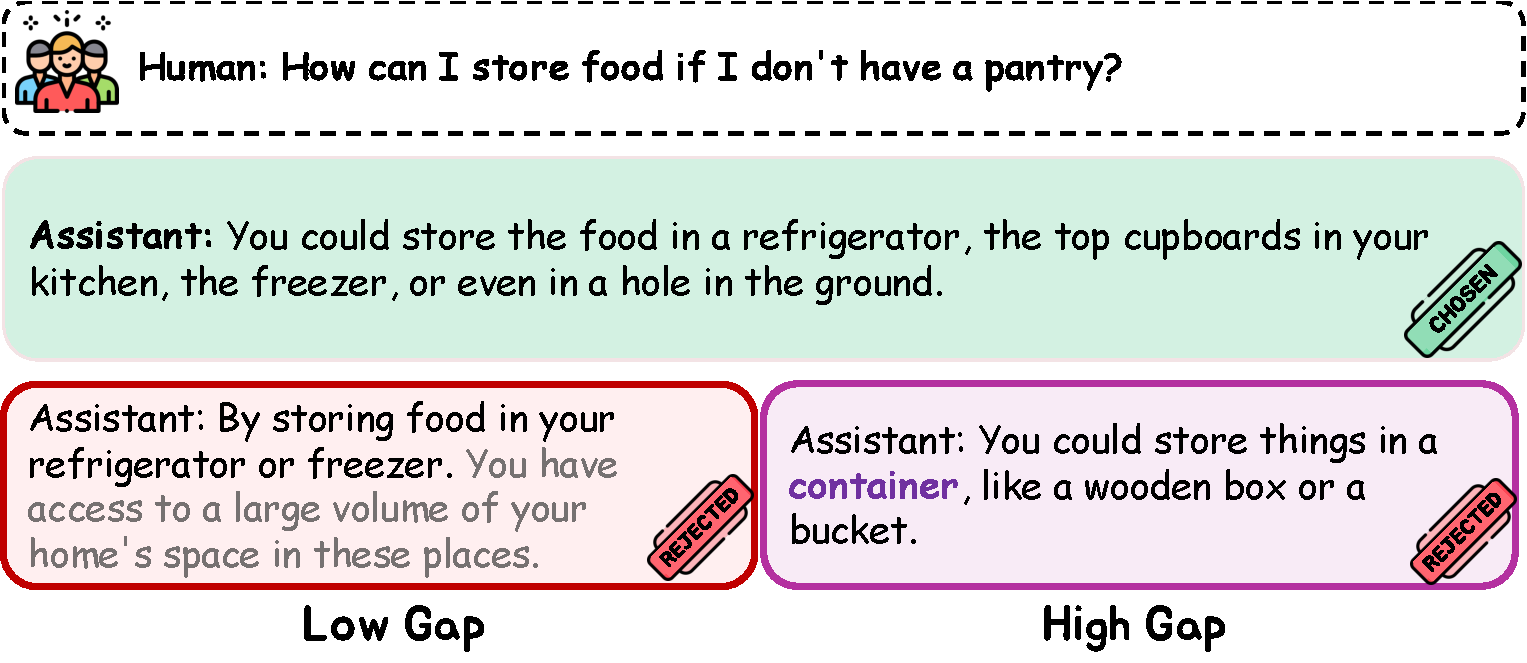
\includegraphics[width=\linewidth]{figs/first_fig_a.pdf}
%       \caption{} % 你可以在这里添加子图标题
%       \label{fig_1_1}
%     \end{subfigure}%
%     \hfill % 这会在子图之间添加一些空间
%     \begin{subfigure}{.3\textwidth}
%       \centering
%       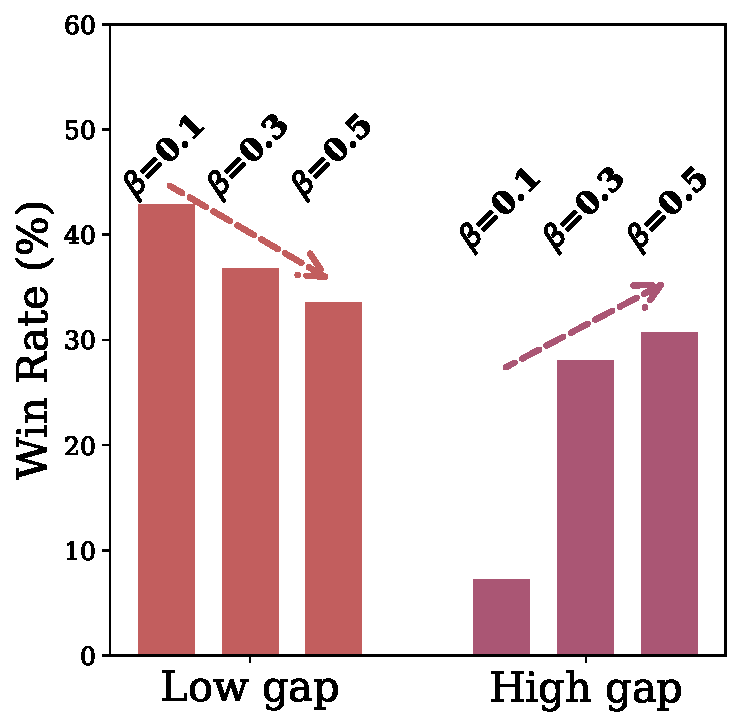
\includegraphics[width=\linewidth]{figs/first_fig.pdf}
%       \caption{} % 同样,为第二个子图添加标题
%       \label{fig_1_2}
%     \end{subfigure}
%     \caption{
%     \textbf{(\ref{fig_1_1}) Pairwise Data: Low vs. High Gap}: `Low gap' denotes closely similar chosen and rejected examples—typically high-quality, informative pairs. `High gap' signifies larger differences, implying less similarity between the paired samples.
%     \textbf{(\ref{fig_1_2}) Influence of Data Quality on $\beta$ Selection:} Pythia1.4b's performance on the HH dataset reveals a distinct trend: for `Low gap' , a higher $\beta$ reduces win rate, whereas for `High gap', an increased $\beta$ improves it.}
%     \label{fig:combined}
% \end{figure}




% ====
% Aligning Large Language Models (LLMs) \cite{GPT4,llama2,GPT4_2} with human feedback has been successfully used to make generations more helpful, factual, and ethical, among other desiderata \cite{instructGPT}.
% The alignment of Large Language Models (LLMs) with human feedback, as explored in works like GPT-4 and LLaMA-2 \cite{GPT4,llama2,GPT4_2}, has marked a significant advancement in generating responses that are more helpful, factual, and ethical \cite{instructGPT}. Among the various alignment strategies, Reinforcement Learning from Human Feedback (RLHF) \cite{instructGPT} is a notable method that refines LLMs using the Proximal Policy Optimization (PPO) algorithm \cite{PPO}.  
% While effective, the RLHF pipeline is significantly less stable and more memory-demanding than supervised learning.

% Recently, Direct Preference Optimization (DPO) \cite{DPO} provides a promising alternative to RLHF, leveraging the mapping between the reward function and the optimal policy to bypass the need for reinforcement learning and explicit reward model learning. The training objective guides the policy model to prefer the human-preferred response $\yb_{w}$ over the reference response $\yb_{l}$. The $\beta$ value is a hyperparameter that controls the deviation from the base reference policy $\piref$. A smaller $\beta$ value leads to a more aggressive update, while a larger $\beta$ value leads to a more conservative update:
% \begin{align*}
%     \EE_{\xb,\yb_{w},\yb_{l}} [-\log \sigma \big(
%     \beta \big[
%     \log \big(\frac{\pi_{\btheta}(\yb_{w}|\xb)}{\pi_{\text{ref}}(\yb_{w}|\xb)}\big)
%     -
%     \log \big(\frac{\pi_{\btheta}(\yb_{l}|\xb)}{\pi_{\text{ref}}(\yb_{l}|\xb)}\big)
%     \big]
%     \big)].
% \end{align*}
% Interestingly, both the selection of the $\beta$ parameter and the quality of pairwise data ($\yb_{w},\yb_{l}$) have drawn much less attention in DPO. 
% Often, the $\beta$ value is typically set to a fixed value, such as $0.1$. But, the generative performance of DPO exhibits a marked sensitivity to the parameter $\beta$, as illustrated in Figure \ref{fig_1_2} (red bars). Notably, when $\beta$ is increased from 0.1 to 0.5, we observe a decline in the win rate from 42\% to 33\%. And the optimal selection of $\beta$ is subject to shift due to variations in data quality (purple bars in \ref{fig_1_2}). For alignment, informative and high quality pairwise data are intuitively those pairs that are mapped nearby (low gap between $\yb_{w}$ and $\yb_{l}$) but should be far apart. By comparing pairs of ($\yb_{w},\yb_{l}$) at different levels of gap (low gap vs. high gap), it is observed that the optimal value of $\beta$ alters correspondingly. Consequently, given the presence of variability in data quality (i.e., outliers) in real-world scenarios, \emph{a fixed $\beta$ is no longer the optimal choice for the DPO.}

% With this motivation, this paper proposes a dynamic $\beta$ that better aligns the DPO process with a broader array of preference data. Achieving this objective introduces two salient challenges: 
% (1) Attributing an instance-wise $\beta$ to each paired example introduces optimization instabilities. Traditional DPO approaches consider $\beta$ assignment at a population level, yet instance-level adjustments—per existing literature—suffer from poor training stability. To tackle this issue, our approach involves adopting a strategy that dynamically assigns $\beta$ at the batch level.
% (2) Setting $\beta$ on a batch-level necessitates consideration of outliers' impact. For a more accurate estimation of an optimal $\beta$ corresponding to a batch, the presence of outliers is an issue that warrants focused attention and resolution. 
% To address the aforementioned challenges, we introduce a dual optimization strategy that encompasses two key tactics:
% \begin{itemize}[leftmargin=*]
%     \item \textbf{The $\beta$ is determined by the quality of pairwise data.} In scenarios characterized by high-quality data (Low Gap), the $\beta$ should be set lower to encourage updates to the policy model. Conversely, for instances marked by a high gap—indicative of lower quality data—the policy model's stance should be more conservative to avoid overfitting. Herein, the dynamic $\beta$ is applied at the batch level, thereby ensuring the stability of the training process.
%     \item \textbf{The data should undergo a filtering process utilizing the benchmarked $\beta$.} This measure is aimed at mitigating the impact of outliers on the estimation of batch-level $\beta$.
% \end{itemize} 

% We sum up our contributions as follows. (1) we pioneer in investigating the relationship between the $\beta$ parameter and the quality of pairwise data. (2) we introduce a novel dynamic $\beta$ approach tailored to the quality of pairwise data. (3) Through empirical evaluation, we demonstrate that our dynamic $\beta$ approach markedly improves performance across a variety of settings and model sizes.
